\begin{subsection}{Systems of Differential Equations}

\begin{frame}{Self 
Propulsion on Uneven Terrain}

\begin{align*}
\frac{d}{dt} \begin{pmatrix}\vec{x}\\\vec{v}\end{pmatrix} = \begin{pmatrix}\vec{v}\\ \hat{\vec{v}} \Big[ \frac{c}{\norm{\vec{v}}} - a \norm{\vec{v}} + \frac{\norm{\vec{v}}^2 - b \vec{v} \cdot \nabla s}{\sqrt{\norm{\vec{v}}^2 + (\vec{v} \cdot \nabla s)^2}} \Big] \end{pmatrix}
\end{align*}

\begin{columns}[T,onlytextwidth]

\column{0.45\textwidth}
\small{
\begin{itemize}
    \item ants choose walking speed to expend constant power {\scriptsize\cite{holt_locomotion_2012}}
    \item gravity opposes uphill movement, aids downhill movement
    \item severe incline/decline decreases overall efficiency of ant movement
    % \item $a$, $b$, $p$, constants governing this effect, were fitted using Matlab's \texttt{lsqcurvefit}
\end{itemize}
}
\column{0.1\textwidth}
\column{0.45\textwidth}
 \begin{figure}
    	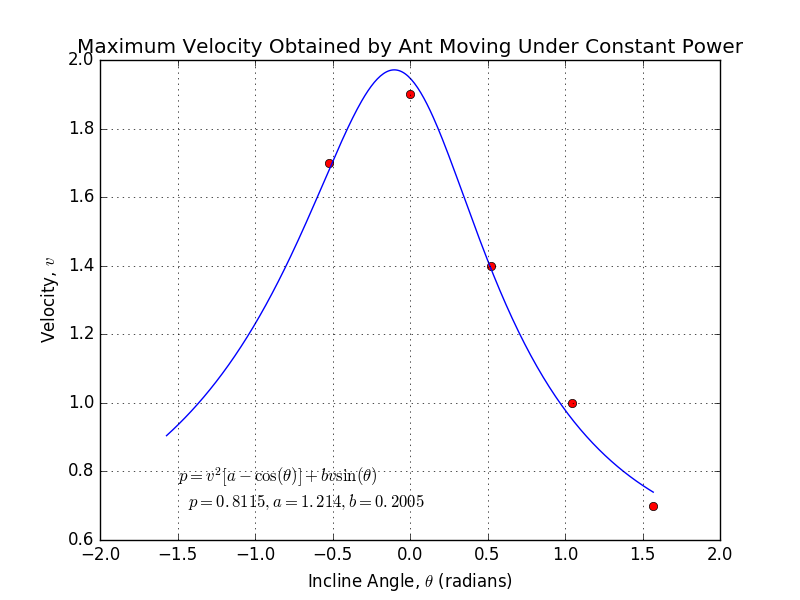
\includegraphics[width=\textwidth]{images/const_power_velocity}
        \caption{Ant velocity under constant power on inclined terrain}
    \end{figure}
\end{columns}
\end{frame}

\end{subsection}
